\chapter{Ergebnisse und Diskussion}
\label{sec:Ergebnisse und Diskussion}

In diesem Kapitel werden die Ergebnisse der analytischen Berechnungen nach Inglis mit der Finite-Elemente-Simulation verglichen, um die Genauigkeit des FE-Modells zu validieren. Im Folgenden werden die wichtigsten Erkenntnisse und Abweichungen diskutiert.

\section{Analytische Berechnungen}
\label{Analytische Berechnung}

Die theoretische Grundlage bildet die Lösung nach Inglis für eine unendlich ausgedehnte Scheibe. Unter Berücksichtigung der Halbachsen ${a = 6\,\mathrm{mm}}$ (vertikal) und ${b = 3\,\mathrm{mm}}$ (horizontal) sowie der Nennspannung ${\sigma_0 = 100\,\mathrm{MPa}}$ ergibt sich die maximale Kerbspannung am Lochrand zu:
\begin{equation}
    \sigma_{xx}^{\mathrm{P}} = 100\,\mathrm{MPa} \cdot \left( 1 + \frac{2 \cdot 6\,\mathrm{mm}}{3\,\mathrm{mm}} \right) = 500\,\mathrm{MPa}.
\end{equation}

\section{Vergleich der Diskretisierungsstrategien}
\label{sec:Vergleich der Diskretisierungsstrategien}

Die Simulationsergebnisse verdeutlichen die hohe Sensitivität der berechneten Spannungsspitzen gegenüber dem gewählten Mesh-Layout und der Elementformulierung.
\begin{itemize}
    \item \texttt{Kuhn\_A2-2\allowbreak \_lin-unseeded.odb}: Die Verwendung eines groben Netzes \sfigref{fig:lin-unseeded_S11} führt zu einer signifikanten Unterschätzung der Kerbspannung auf ca. ${425\,\mathrm{MPa}}$ (Abweichung von ${15\,\%}$). Die Detailansicht (\figref{fig:lin-unseeded_S11_detail}) zeigt eine stufige Darstellung der Spannungsgradienten, da die linearen Formfunktionen den steilen Abfall der Spannung im Kerbbereich nicht adäquat auflösen können.
    \item \texttt{Kuhn\_A2-2\_lin-seeded.odb}: Trotz der lokalen Verfeinerung am Lochrand (\figref{fig:lin-seeded_S11} und \figref{fig:lin-seeded_S11_detail}) verbessert sich das Ergebnis nur geringfügig auf ca. ${429\,\mathrm{MPa}}$. Dies belegt, dass bei hohen Spannungsgradienten und gekrümmten Geometrien eine reine Erhöhung der Elementanzahl bei linearen Elementen (ohne parabolische Formfunktionen) nur langsam zur Konvergenz führt.
    \item \texttt{Kuhn\_A2-2\_quad-seeded\_V1.odb}: Mit dem Wechsel auf voll integrierte quadratische Elemente \texttt{CPS8} und einem Bias-Seeding am Lochumfang wird ein Spitzenwert von ca. ${494\,\mathrm{MPa}}$ erreicht. (\sfigref{fig:quad-seeded_V1_S11}) Dies entspricht einer Abweichung von weniger als ${1.2\,\%}$ zum analytischen Wert. Die Detailansicht in \figref{fig:quad-seeded_V1_S11_detail} zeigt einen harmonischen, weichen Spannungsübergang, was auf eine hohe numerische Güte der Lösung hindeutet. Die geringe Restabweichung lässt sich auf den Einfluss der endlichen Plattenbreite im Vergleich zum unendlichen analytischen Modell zurückführen.
    \item \texttt{Kuhn\_A2-2\_quad-seeded\_V2.odb}: Durch eine Einführung des Single-Bias an den Quadrantenteilenden und Außenkanten (\sfigref{fig:quad-seeded_V2_S11}) steigt die Kerbspannung auf ca. ${627\,\mathrm{MPa}}$ (Abweichung von ca. ${25\,\%}$). Die Detailanalyse in \figref{fig:quad-seeded_V2_S11_detail} offenbart hier einen numerischen Fehler: Die Elemente an der Kerbspitze werden durch das extreme Seeding geometrisch so stark verzerrt, dass sie mathematisch kollabieren. Dies führt bei der Extrapolation von den Integrationspunkten zu den Knoten zu physikalisch unsinnigen Spannungsspitzen.
\end{itemize}

\begin{figure}
    \centering

    \begin{subfigure}{.55\textwidth}
        \centering
        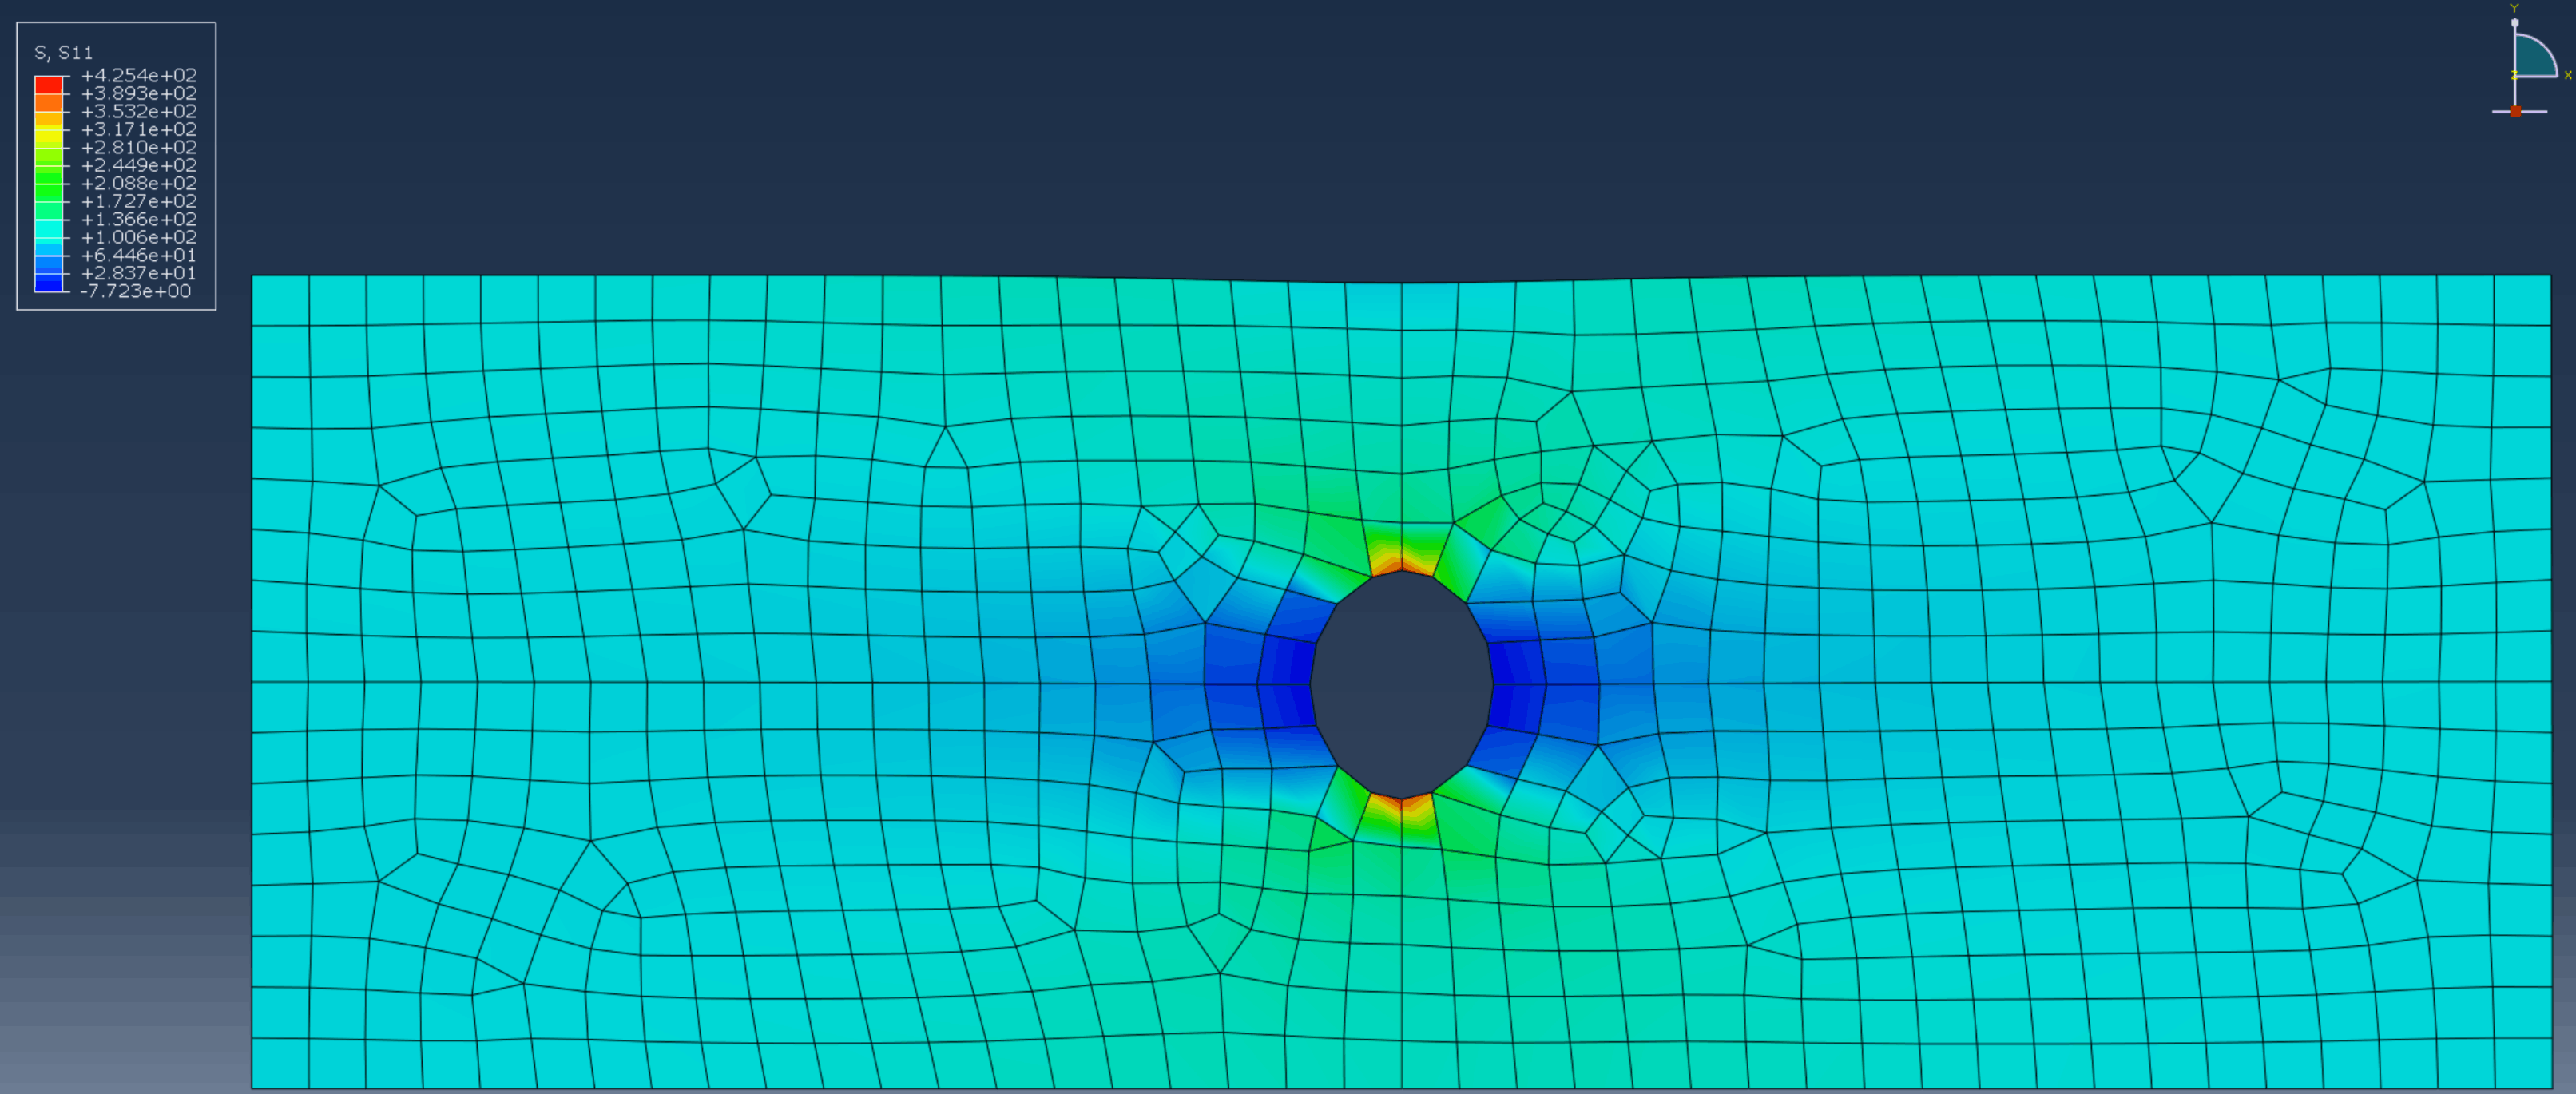
\includegraphics[width=\textwidth]{_ltx/Kuhn_A2-2_lin-unseeded_S11.png} % Datei für unseeded S11
        \caption{${S11}$ der Scheibe mit linearen Elementen und ungesteuertem Seeding}
        \label{fig:lin-unseeded_S11}
    \end{subfigure}

    %\hfill % Schiebt die Bilder auseinander, damit sie nebeneinander stehen
    \vspace{.5em} % Optional: Zusätzlicher vertikaler Abstand zwischen den Bildern
    \begin{subfigure}{.55\textwidth}
        \centering
        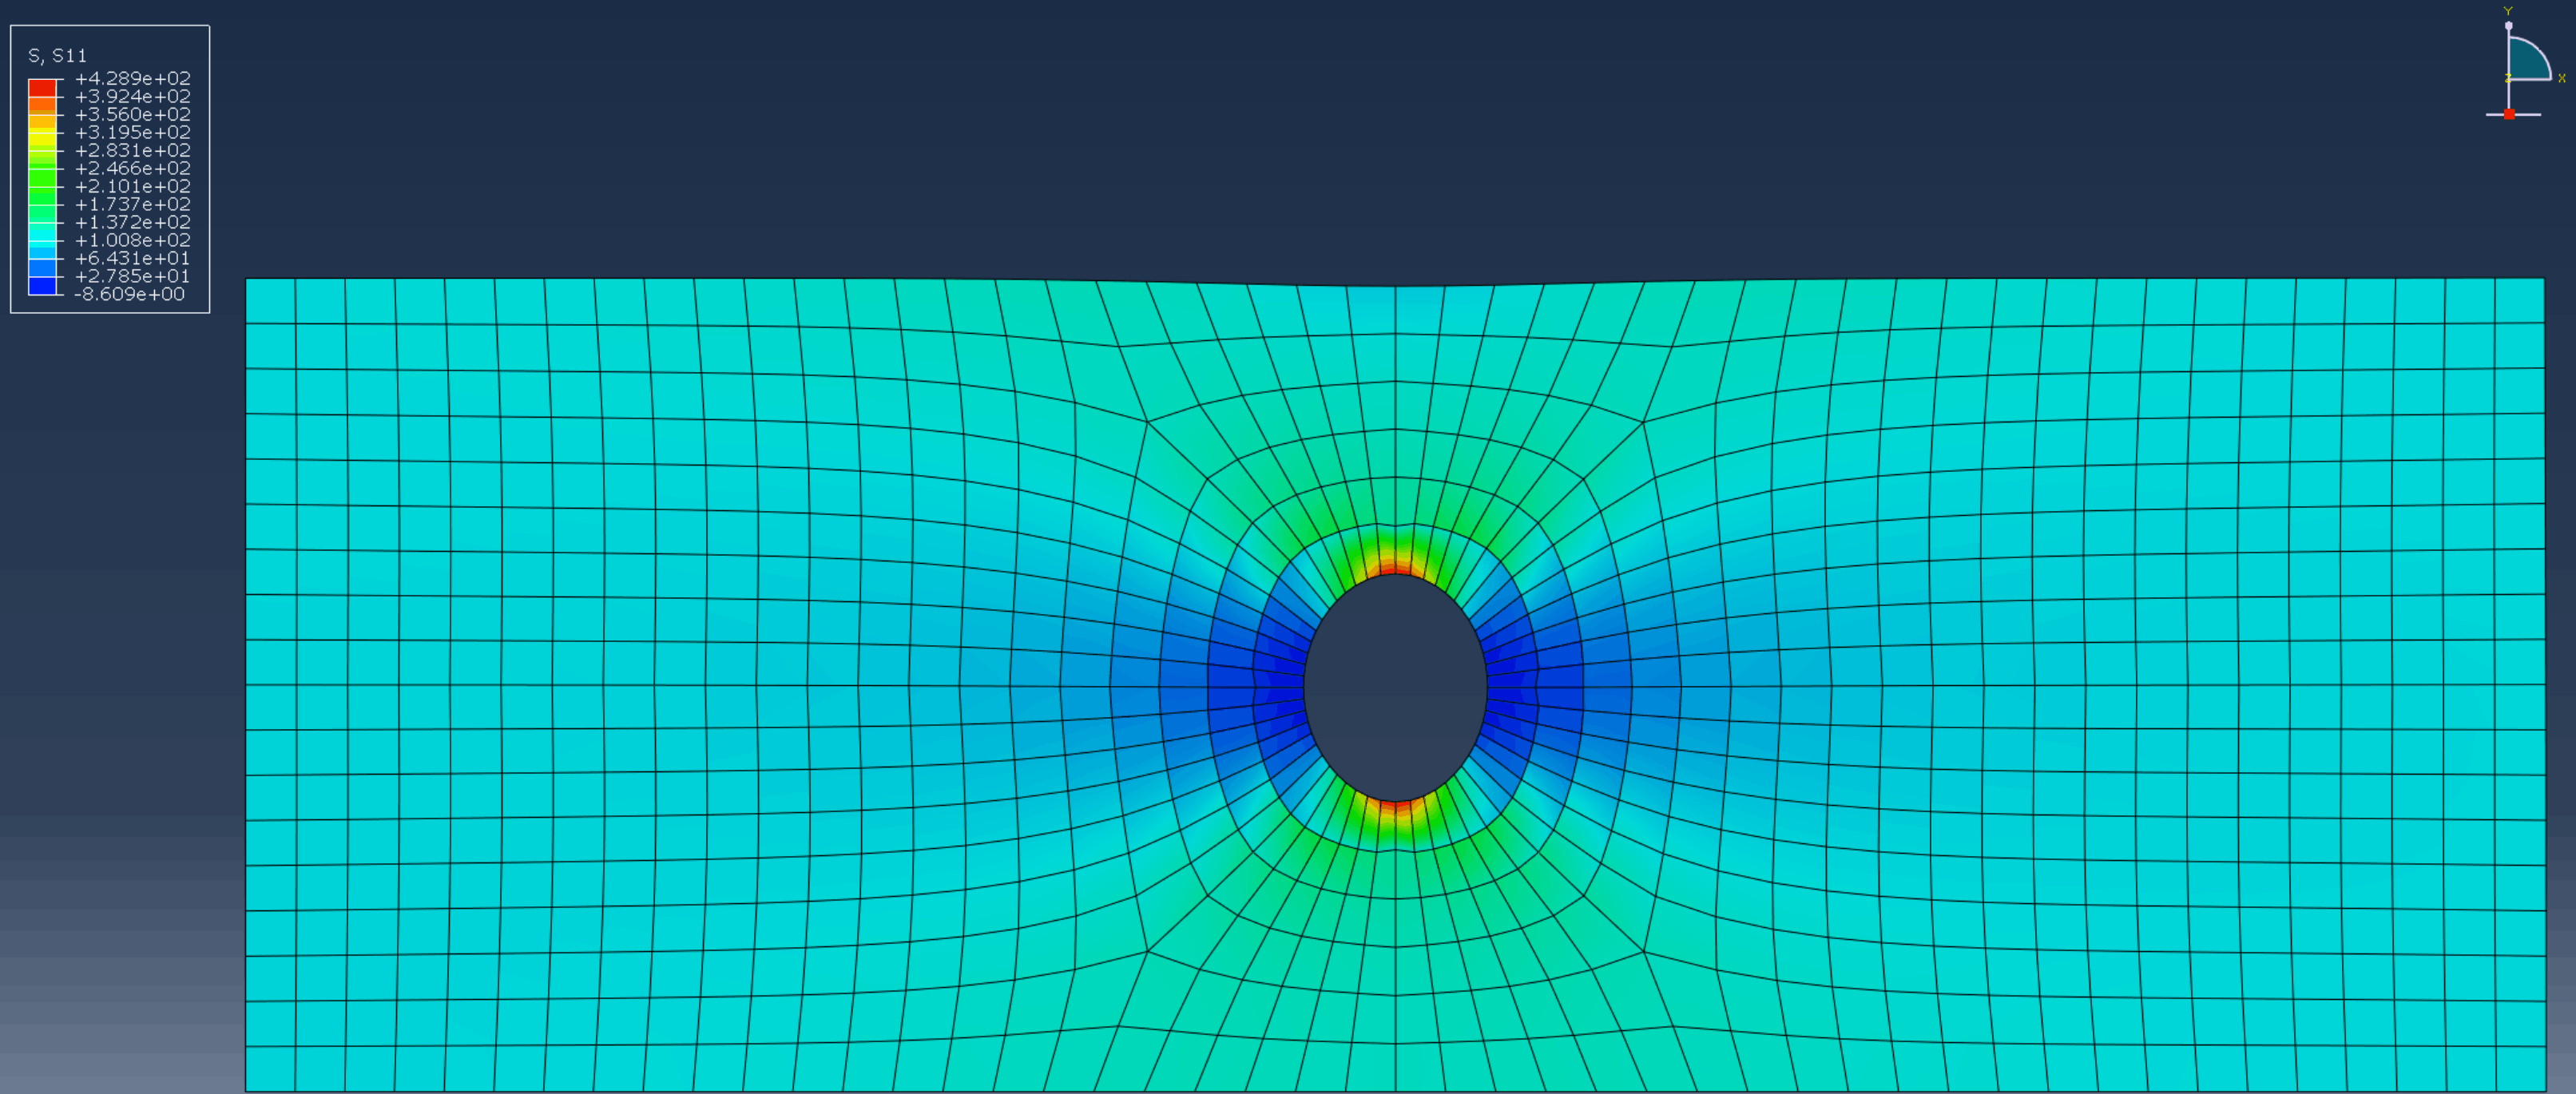
\includegraphics[width=\textwidth]{_ltx/Kuhn_A2-2_lin-seeded_S11.png} % Datei für seeded S11
        \caption{${S11}$ der Scheibe mit linearen Elementen und gesteuertem Seeding}
        \label{fig:lin-seeded_S11}
    \end{subfigure}

    \vspace{.5em} % Optional: Zusätzlicher vertikaler Abstand zwischen den Bildern

    \begin{subfigure}{.55\textwidth}
        \centering
        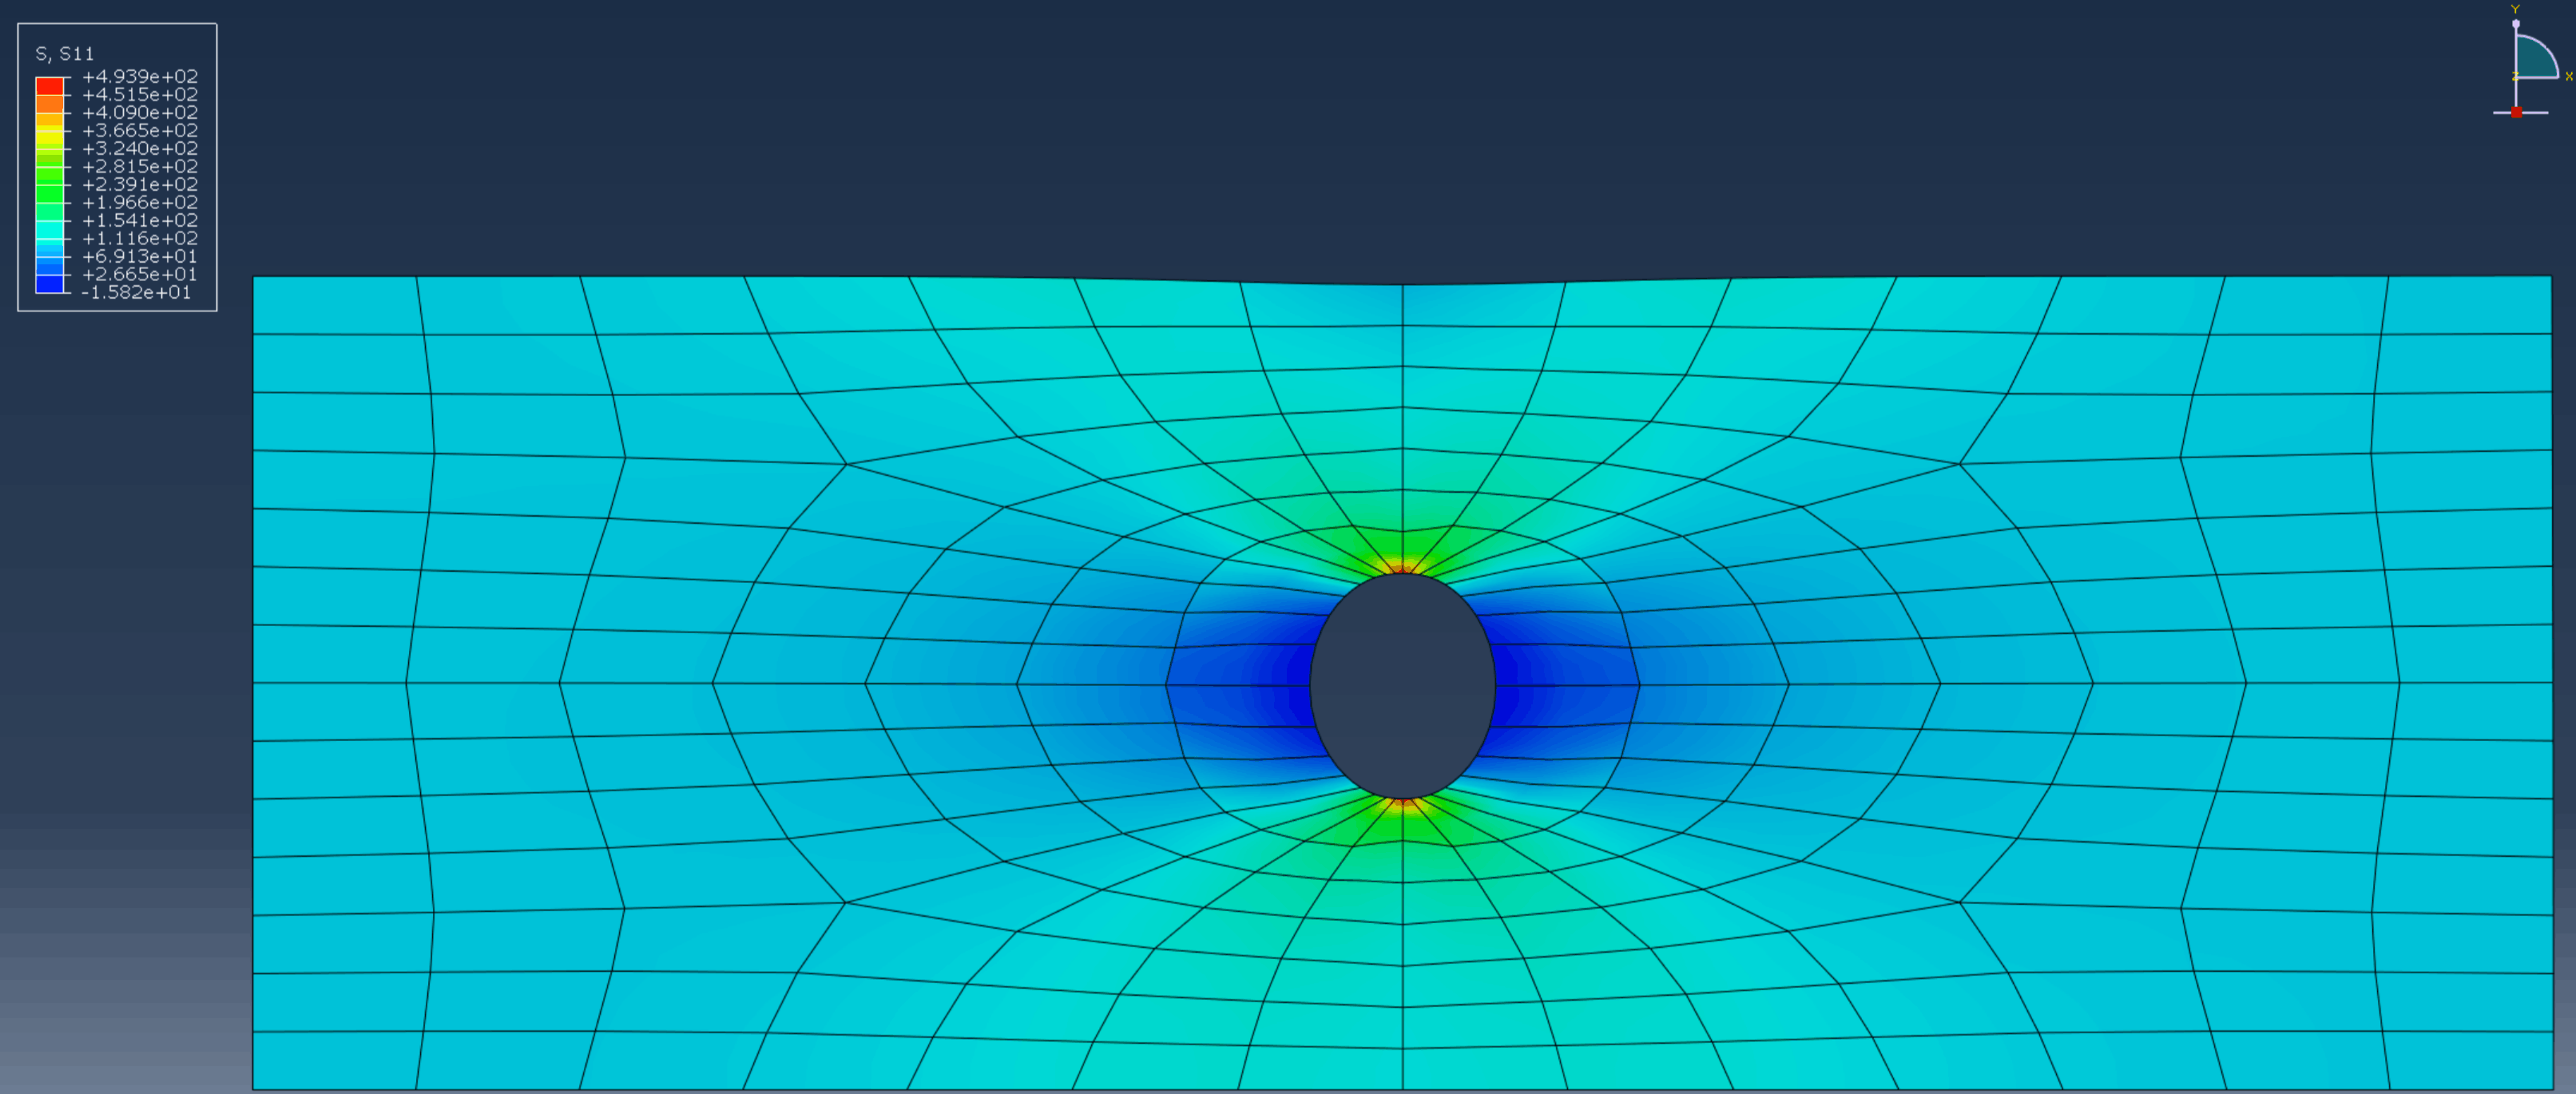
\includegraphics[width=\textwidth]{_ltx/Kuhn_A2-2_quad-seeded_V1_S11.png} % Datei für quad seeded mesh V1
        \caption{${S11}$ der Scheibe mit quadratischen Elementen und gesteuertem Seeding V1}
        \label{fig:quad-seeded_V1_S11}
    \end{subfigure}

    %\hfill % Schiebt die Bilder auseinander, damit sie nebeneinander stehen
    \vspace{.5em} % Optional: Zusätzlicher vertikaler Abstand zwischen den Bildern
    \begin{subfigure}{.55\textwidth}
        \centering
        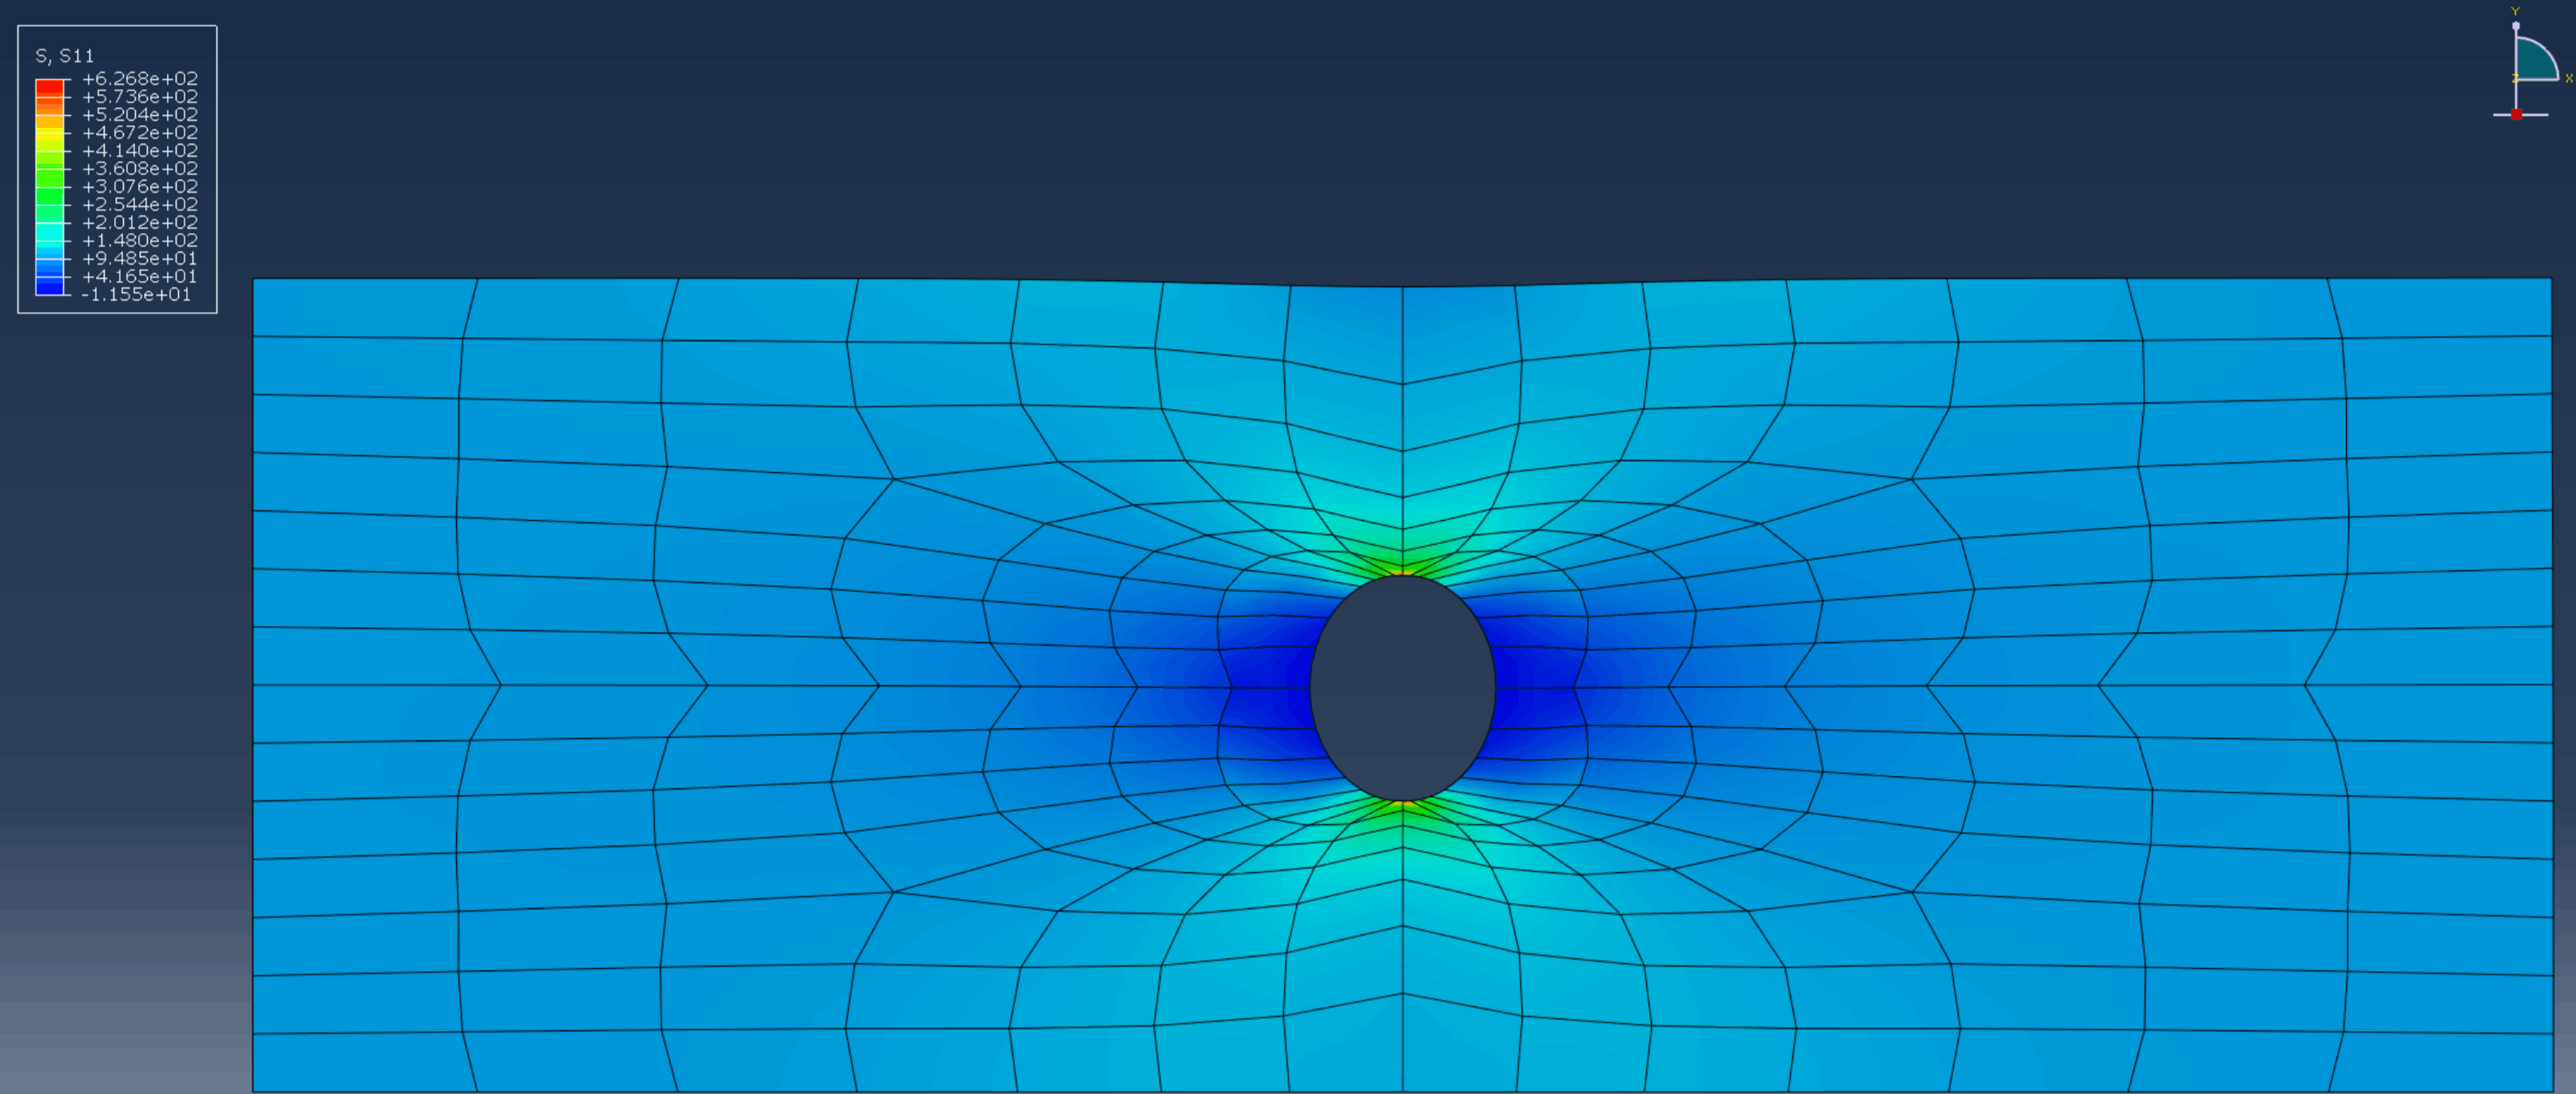
\includegraphics[width=\textwidth]{_ltx/Kuhn_A2-2_quad-seeded_V2_S11.png} % Datei für quad seeded mesh V2
        \caption{${S11}$ der Scheibe mit quadratischen Elementen und gesteuertem Seeding V2}
        \label{fig:quad-seeded_V2_S11}
    \end{subfigure}

    \caption{${S11}$ der Lochscheibe in den verschiedenen Iterationen der Netzoptimierung}
    \label{fig:S11 Lochscheibe}
\end{figure}

\begin{figure}[htbp]
    \centering

    \begin{subfigure}{0.48\textwidth}
        \centering
        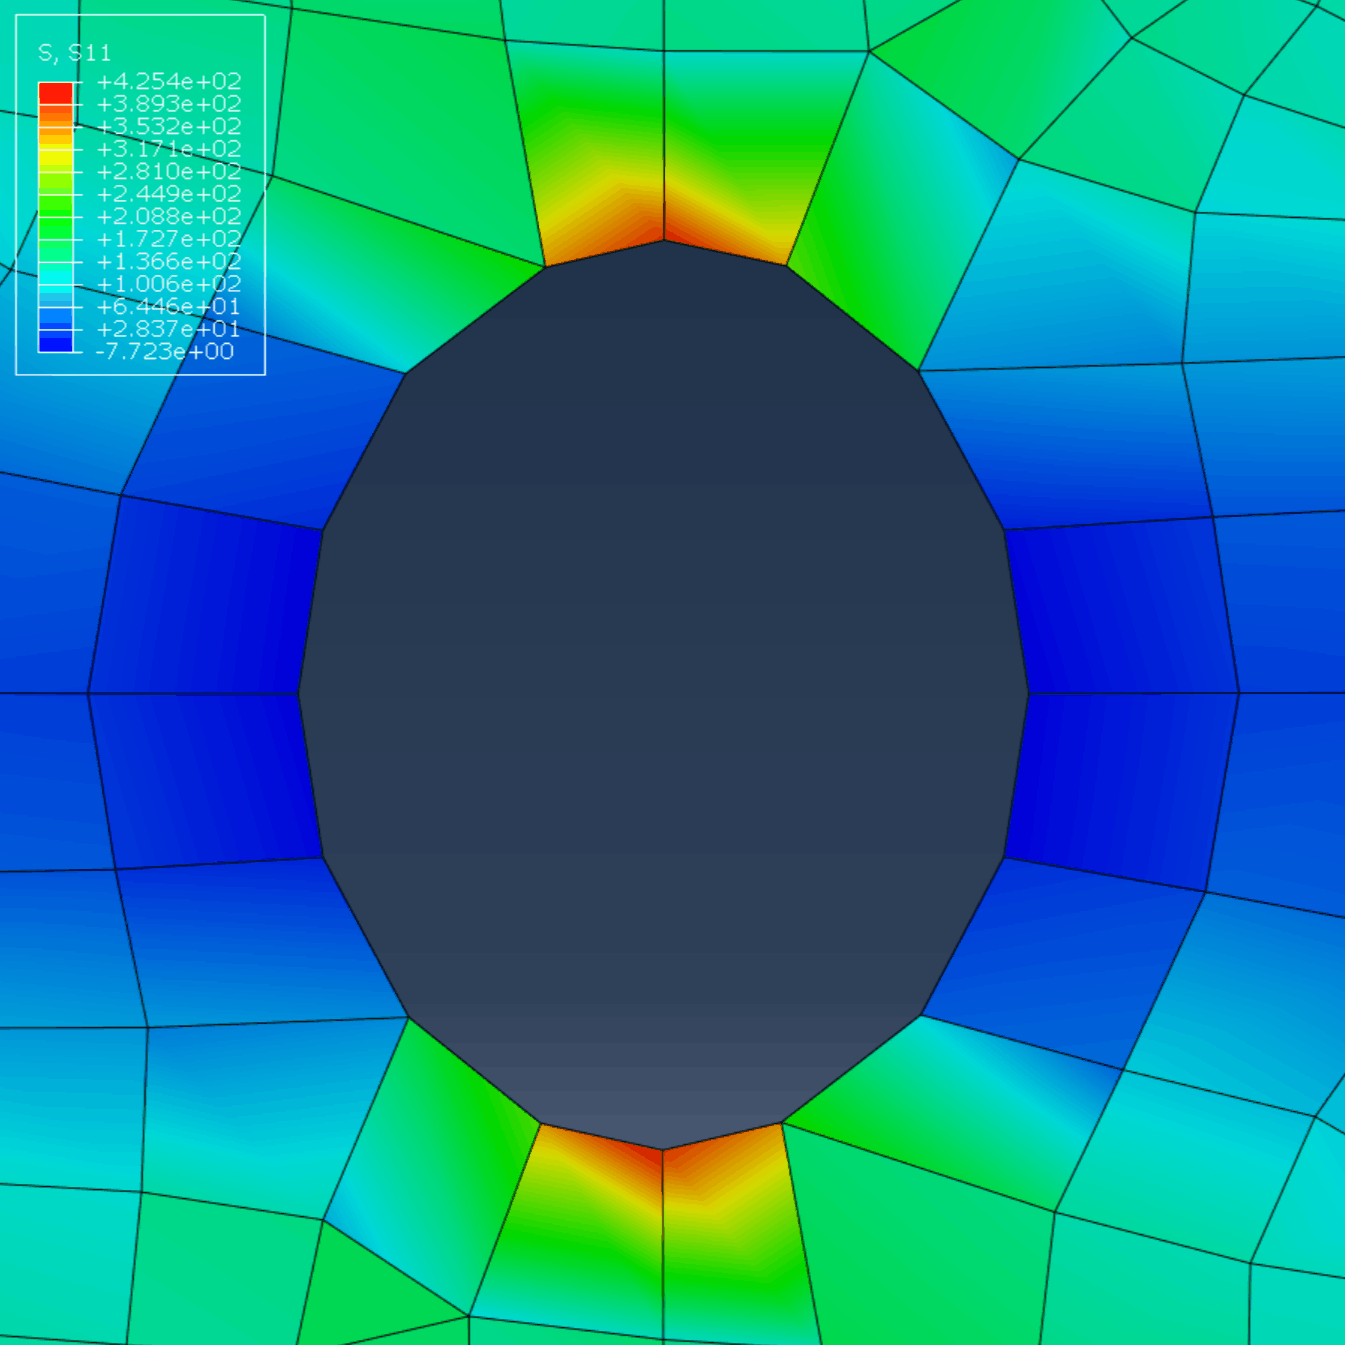
\includegraphics[width=\textwidth]{_ltx/Kuhn_A2-2_lin-unseeded_S11_detail.png} % Datei für unseeded S11 detail
        \caption{Detail ${S11}$ der Scheibe mit linearen Elementen und ungesteuertem Seeding}
        \label{fig:lin-unseeded_S11_detail}
    \end{subfigure}
    \hfill % Schiebt die Bilder auseinander, damit sie nebeneinander stehen
    %\vspace{.5em} % Optional: Zusätzlicher vertikaler Abstand zwischen den Bildern
    \begin{subfigure}{0.48\textwidth}
        \centering
        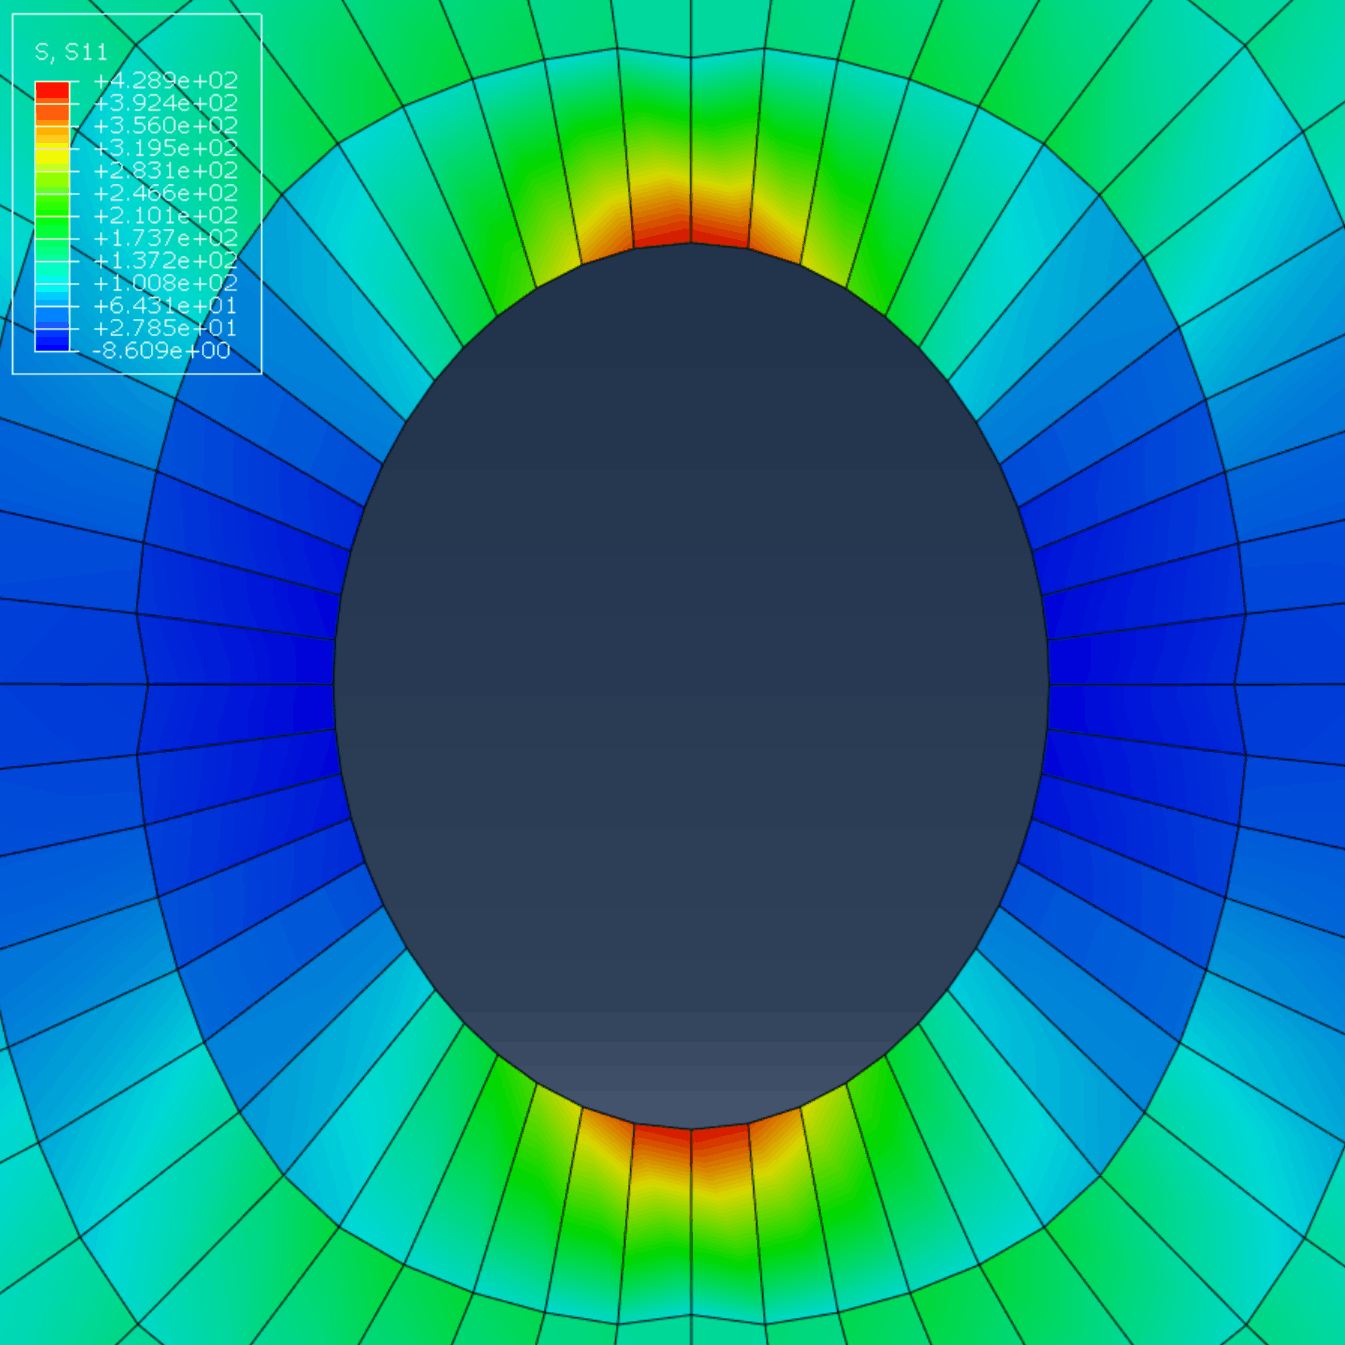
\includegraphics[width=\textwidth]{_ltx/Kuhn_A2-2_lin-seeded_S11_detail.png} % Datei für seeded S11 detail
        \caption{Detail ${S11}$ der Scheibe mit linearen Elementen und gesteuertem Seeding}
        \label{fig:lin-seeded_S11_detail}
    \end{subfigure}

    \vspace{.5em} % Optional: Zusätzlicher vertikaler Abstand zwischen den Bildern

    \begin{subfigure}{0.48\textwidth}
        \centering
        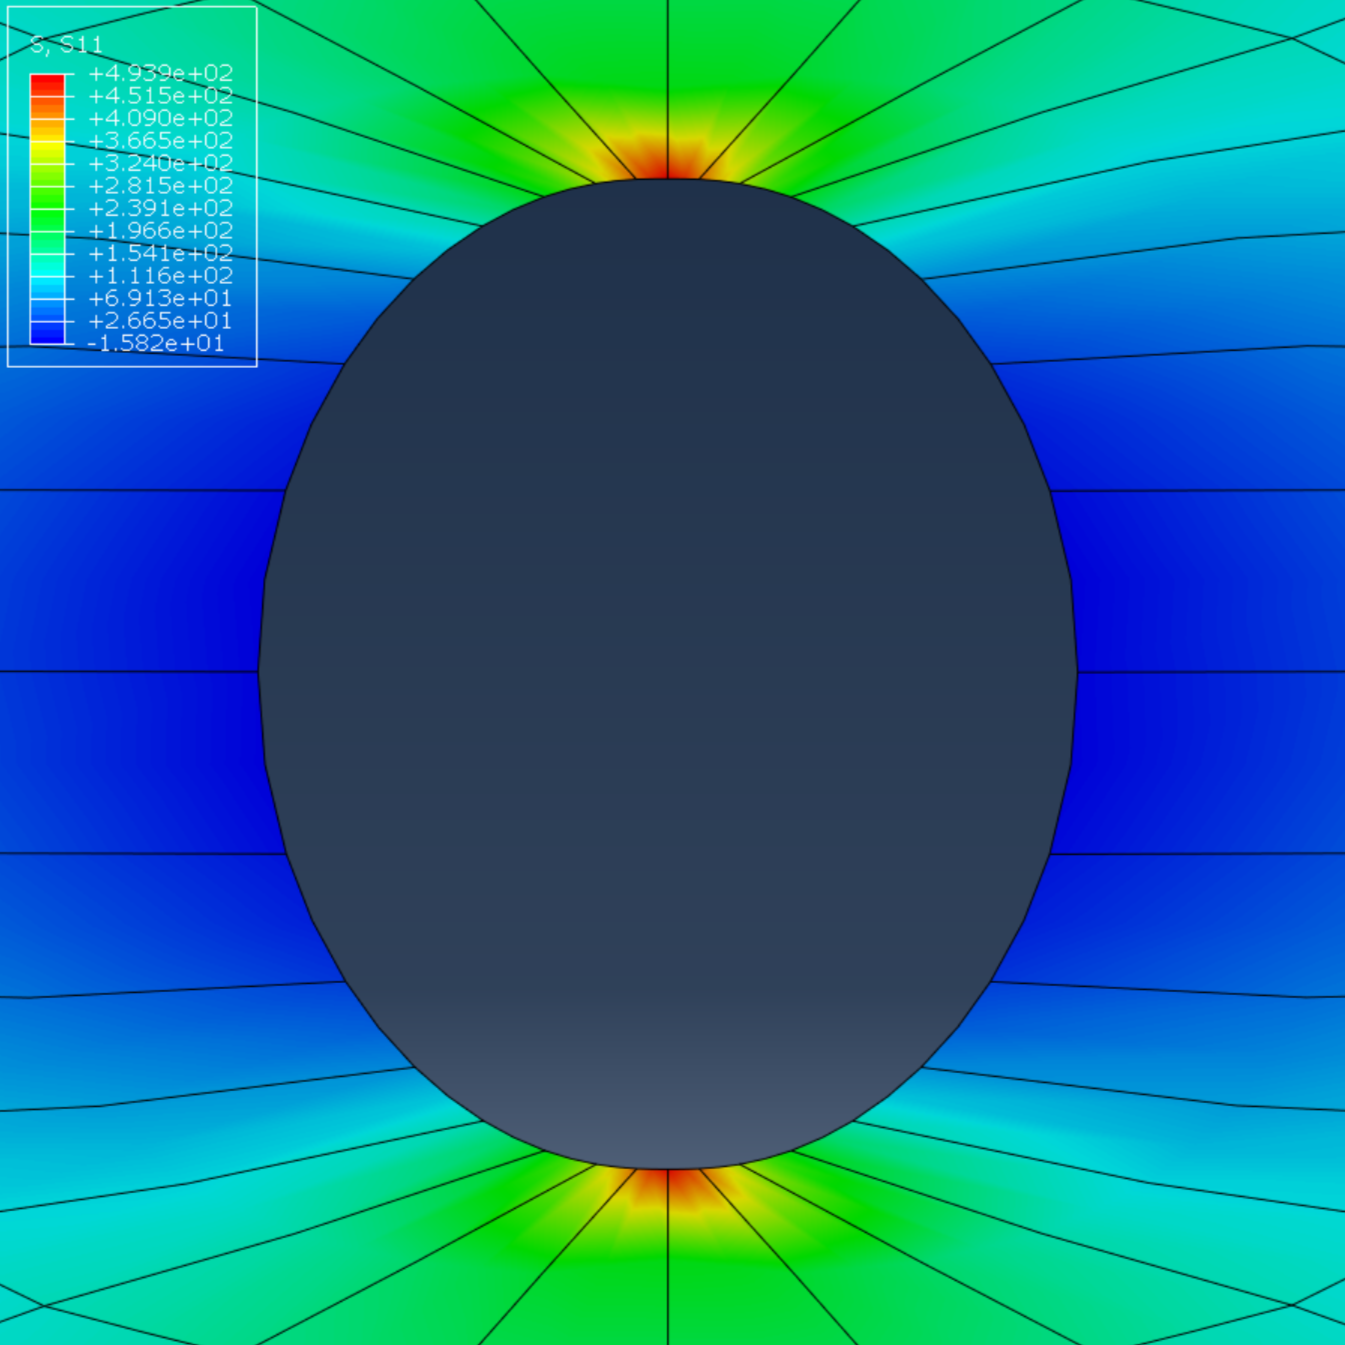
\includegraphics[width=\textwidth]{_ltx/Kuhn_A2-2_quad-seeded_V1_S11_detail.png} % Datei für quad seeded mesh V1 detail
        \caption{Detail ${S11}$ der Scheibe mit quadratischen Elementen und gesteuertem Seeding V1}
        \label{fig:quad-seeded_V1_S11_detail}
    \end{subfigure}
    \hfill % Schiebt die Bilder auseinander, damit sie nebeneinander stehen
    %\vspace{.5em} % Optional: Zusätzlicher vertikaler Abstand zwischen den Bildern
    \begin{subfigure}{0.48\textwidth}
        \centering
        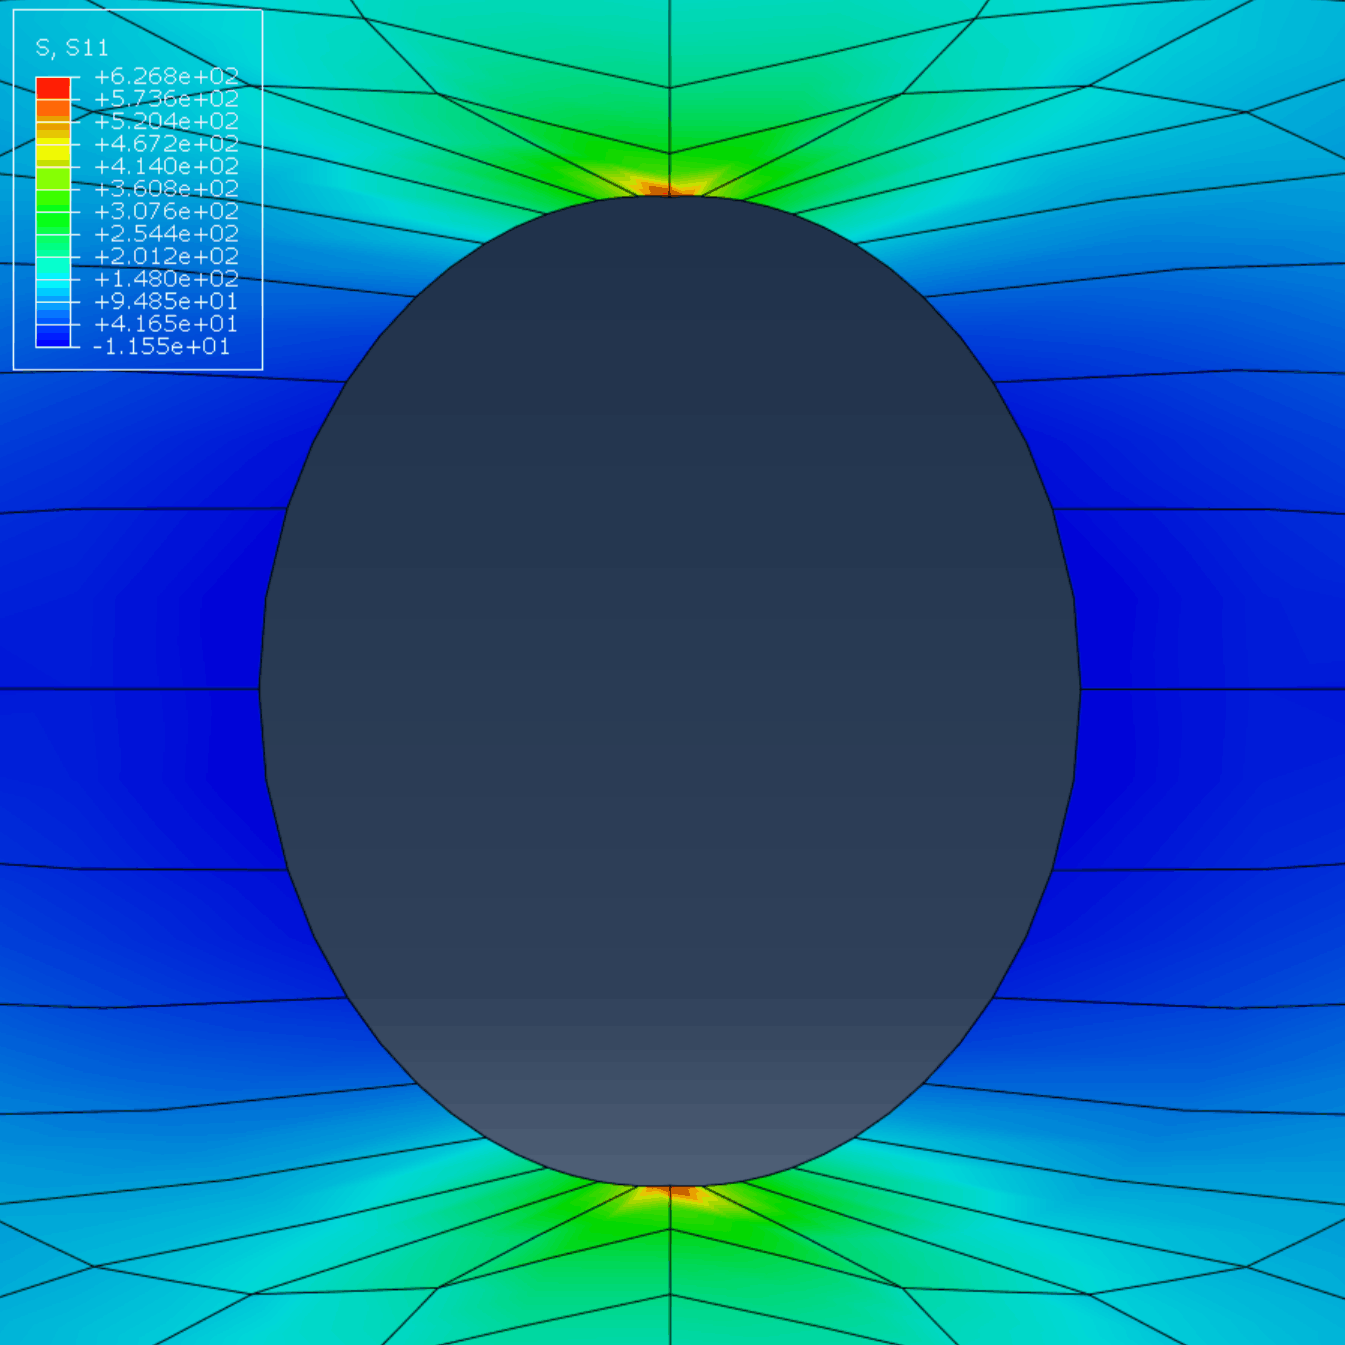
\includegraphics[width=\textwidth]{_ltx/Kuhn_A2-2_quad-seeded_V2_S11_detail.png} % Datei für quad seeded mesh V2 detail
        \caption{Detail ${S11}$ der Scheibe mit quadratischen Elementen und gesteuertem Seeding V2}
        \label{fig:quad-seeded_V2_S11_detail}
    \end{subfigure}

    \caption{Detailansicht ${S11}$ der Lochscheibe in den verschiedenen Iterationen der Netzoptimierung}
    \label{fig: Deatilansicht S11 Lochscheibe}
\end{figure}

\section{Analyse des Spannungsverlaufs entlang des Pfadplots ${A-A}$}
\label{sec:Analyse des Spannungsverlaufs entlang des Pfadplots A-A}

Der für die Version V1 generierte Pfadplot (\sfigref{fig:quad-seeded_V1_S11_path}) entlang des Pfads ${A-A}$ verdeutlicht den Charakter der Spannungskonzentration.
\begin{itemize}
    \item Kerbbereich: An den Scheitelpunkten des elliptischen Lochs (${y = 14\,\mathrm{mm}}$ und ${y = 26\,\mathrm{mm}}$) erreicht die Spannung ihr Maximum von ca. ${494\,\mathrm{MPa}}$.
    \item Gradientenabbau: Ausgehend vom Lochrand fällt die Spannung ${\sigma_{xx}}$ sehr steil ab. Bereits in geringer Entfernung zur Kerbe nähert sich der Verlauf dem ungestörten Spannungszustand an.
    \item Randbereich: An den Außenrändern der Scheibe (${y = 0\,\mathrm{mm}}$ und ${y = 40\,\mathrm{mm}}$) sinkt die Spannung auf Werte nahe der Nennspannung ${\sigma_0}$, was die lokale Begrenztheit des Kerbeinflusses (St. Venantsches Prinzip) bestätigt.
\end{itemize}

\begin{figure}[htbp]
    \centering
    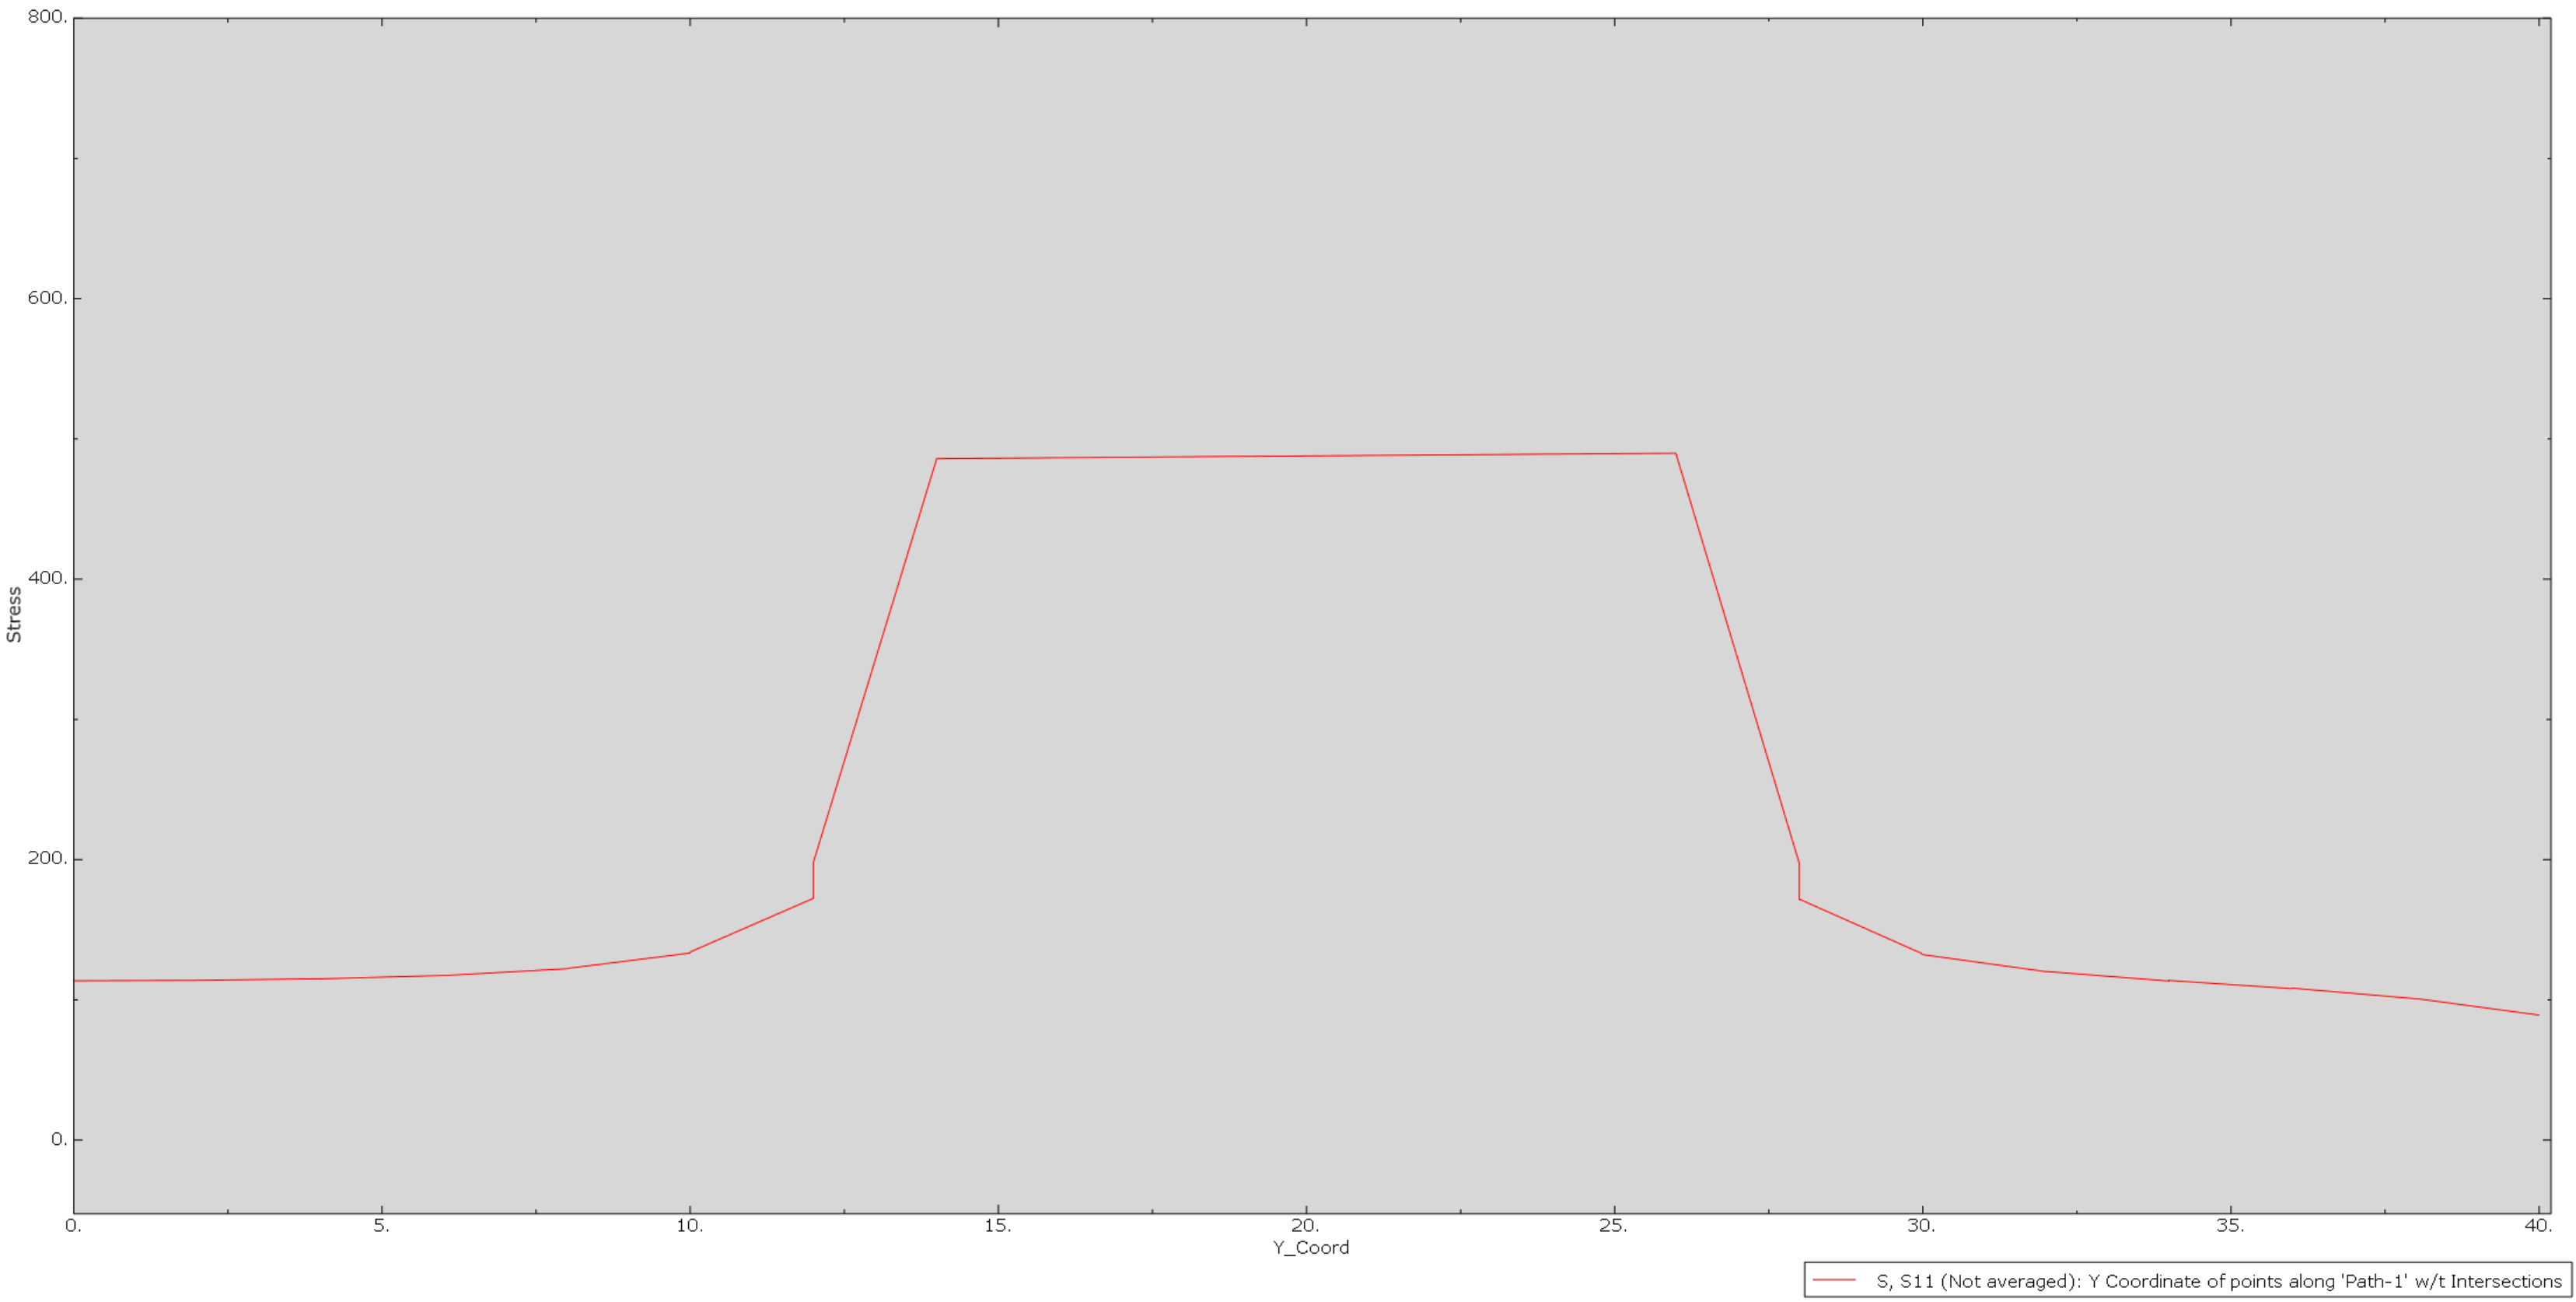
\includegraphics[width=\textwidth]{_ltx/Kuhn_A2-2_quad-seeded_V1_S11-path.png} % Datei für quad seeded S11 path
    \caption{Pfadplot ${A-A}$ der Scheibe mit quadratischen Elementen und gesteuertem Seeding V1}
    \label{fig:quad-seeded_V1_S11_path}
\end{figure}
